\chapter*{مقدّمة}

\vspace{-0.6em}
تحبّ تعلّم البرمجة لكن لا تعرف من أين تبدأ ؟ هذه الدروس لتعليم لغة الـ\textenglish{C}
للمبتدئين قد جُعلت خصّيصاً من أجلك !

\vspace{-0.1em}
لغة الـ\textenglish{C}
هي لغة لا مفرّ منها، أُستلهمَت منها العديد من اللغات الأخرى. تمّ اختراعها في السبعينات و لا تزال مستعملة لحدّ الآن في البرمجة النظامية و عالم الروبوتات. تعتبر لغة الـ\textenglish{C}
لغة معقّدة، لكن إن استطعت تعلّمها ستكوّن لك قاعدة برمجية صلبة !

\vspace{-0.1em}
في هذه الدروس، ستبدأ باكتشاف مبدأ عمل الذاكرة، المتغيرات، الشروط و الحلقات. ثم ستقوم باستعمال كلّ ما تعلّمته في إنشاء واجهات رسومية بالاستعانة بالمكتبة
\textenglish{SDL}
 (ألعاب فيديو، تسجيلات صوتية \dots). أخيراً، ستتعلّم كيف تتعامل مع هياكل البيانات الأكثر شيوعاً من أجل تنظيم المعلومات في الذاكرة : قوائم متسلسلة، مكدّسات، طوابير، جداول تجزئة \dots

\vspace{-0.1em}
التحق بي في هذه الدروس من أجل اكتشاف البرمجة بلغة الـ\textenglish{C} !

\begin{figure}[H]
	\centering
	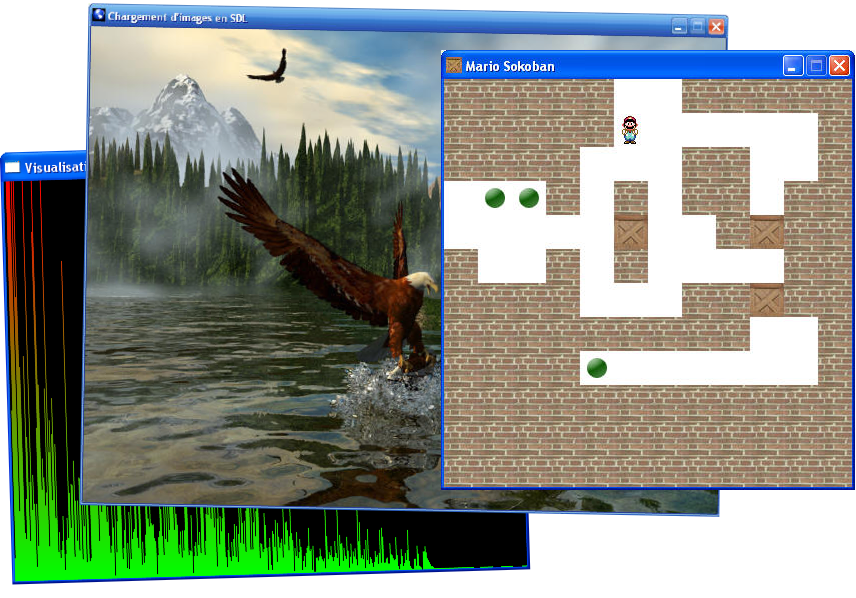
\includegraphics[height=0.4\textheight]{Introduction_original}\\
\small بعض الإنجازات الّتي سنقوم بها في هذا الكتاب
\end{figure}

\vfill
\hfill\parbox{0.3\textwidth}{\centering \textenglish{Mathieu Nebra}\\[0.2em]
مؤسس مشارك لموقع
\href{http://openclassrooms.com/}{\textenglish{OpenClassrooms}}
}
